\documentclass[main.tex]{subfiles}

\begin{document}
\section{Modelli di classificazione pesati}

Essendo interessati all\rq{}identificazione corretta dello {\em shake}, si è scelto di attribuire dei pesi alle classi che penalizzassero quest\rq{}ultima. I pesi sono stati determinati mediante una ricerca sequenziale. Usando come pesi di base le frequenze relative di ciascuna classe, si è diviso il peso della classe {\em shake} secondo una sequenza crescente di valori, normalizzando i pesi delle altre classi in modo da farli sommare a uno. I pesi sono stati scelti in modo da massimizzare l\rq{}accuratezza sotto il vincolo di avere un tasso di veri positivi nella classe {\em shake} pari al $100\%$ nell\rq{}insieme di convalida.

I risultati in termini di accuratezza ottenuti sull\rq{}insieme di convalida sono mostrati in tabella.
\begin{table}[H]
\centering
\caption{Accuratezza per i modelli adattati sull'insieme di validazione.}
\begin{tabular}{cc}
\toprule
      Modello &  Accuratezza \% \\
\midrule
          QDA &          82.20 \\
 Multinomiale &          82.02 \\
          LDA &          68.62 \\
\bottomrule
\end{tabular}
\label{tab:acc_pen}
\end{table}

La classificazione migliore tenendo conto della penalizzazione è ottenuta con l\rq{}analisi discriminante quadratica. Il modello multinomiale scende al secondo posto.

La matrice di confusione per il modello migliore è la seguente.
\begin{figure}[H]
	\centering
	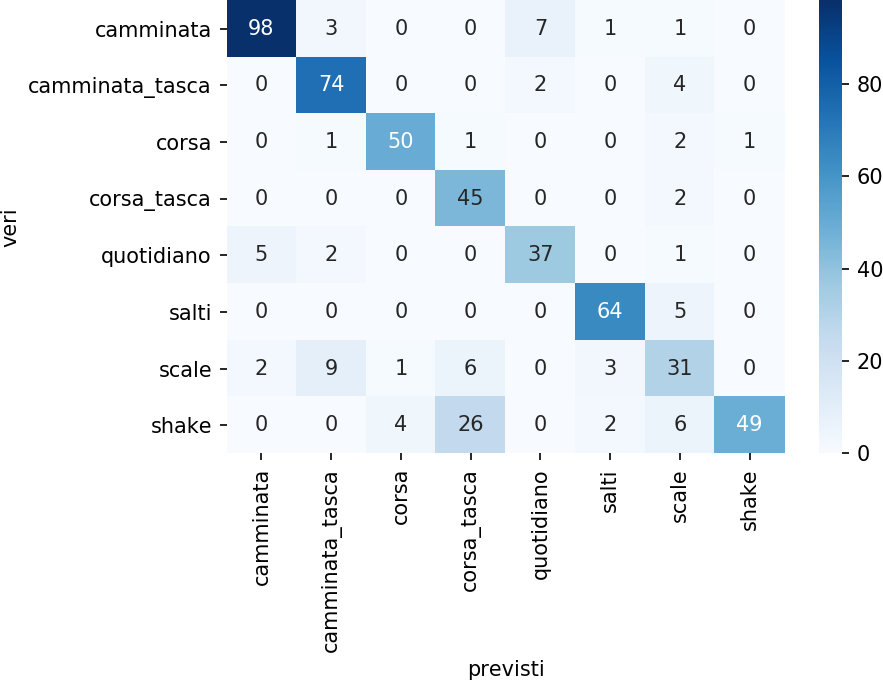
\includegraphics[width=.5\textwidth]{../../figure/confusionMatrix-QDA-penalizzata.png}
	\caption{Matrice di confusione ottenuta con l'analisi discriminante quadratica.}
	\label{fig:qda_pen}
\end{figure}
\end{document}